\chapter{拟采取的研究方法、技术路线、实验方案及其可行性分析}

\section{研究方法与技术路线}

本节介绍通用多FPGA硬件仿真系统REMUS的研究方法与技术路线。REMUS整体技术路线同样遵循上述的多FPGA系统部署的三大步骤：电路划分、结构集成、互联体系。下文将从三大步骤的角度分别进行介绍。

\subsection{模块级抽象策略与自适应粒度电路划分框架实现}

在电路和超图建模方面，首先使用开源综合工具Yosys解析RTL，将其初步转化为Yosys的中间表示，这时后期处理的基础。下一步是关键的预处理，这是实现自适应粒度的核心。如表所示，该算法会递归地遍历模块实例化树，计算每个模块的资源使用情况，并根据预设的资源阈值决定是否展开子模块。该方式能够动态地调整划分的粒度，在使得每个模块的资源使用更加均衡的同时，加快了划分算法的运行速度，不需要展开整个设计，减小了超图划分算法的输入规模。这种自适应的粒度调整机制，使得我们的划分框架能够灵活地适应不同的电路划分需求，在效率和性能之间进行良好的折中。

完成自适应预处理后，需要将设计转化为超图并调用超图划分算法。当输入是一个网表的时候，设计中的每一个实例化都是一个标准库单元，每条连接都是1位长度。每个标准库单元被抽象成为权重相同的超图节点，连接被抽象成为权重相同的超边。对于大规模的设计，转化出来的超图也会十分庞大，这对解析器和算法都提出了性能上的挑战。但这依然存在压缩的空间，因此REMUS提出了模块级的抽象策略。对于层次结构设计，仅扫描顶层的所有实例化和连接。按照连接关系，将所有实例和所有端口转化成顶点，所有的连接抽象成一条超边。此时连接不再以位为单位，而是以线网作为单位。为了实现更好的划分平衡度和真实性，我们为每一个顶点和超边赋予权重。目前顶点的权重是基于综合工具的资源评估结果，超边的权重则是基于连接的位宽。这种赋值权重的方式能很好的适配TritonPart的超图划分算法，节点的权重类型可以是一个向量，用于描述该模块所消耗的各种资源的数目。这能够使得划分结果从不同的资源占用的角度看都足够均衡。

\subsection{集成控制器的实现与仿真就绪单元}

在REMUS的集成步骤中，需要实现划分集成与扫描链集成。划分集成采用DUOHUAFEN的LI-TDM跨FPGA边界接口，而扫描链集成采用REMU的方案。尽管是已有可用的两个方案，然而REMU的扫描链控制器与 LI-TDM 控制器语义冲突，无法直接复用。REMUS需要设计了新的统一控制逻辑，实现多FPGA的同步启停、扫描链双向数据传输以及周期级精确状态捕获。

如图\ref{fig::LI-TDM}所示，LI-TDM的控制器会根据系统时钟和数据传输桥生成一个新的时钟用于控制所有时序逻辑，保证划分子设计在计算完全部的组合逻辑后才前进一个时钟周期。扫描链的控制器则更为复杂，它会生成运行时钟和扫描时钟，两个时钟都需要连接到所有时序器件中，而它的输入是系统时钟和设计中抽取的Trace信号。Trace信号是REMU流程生成的，用于在指定监视的信号发生变化时，停止设计运行。为此，REMUS将LI-TDM的生成的运行时钟转化一个使能信号，将使能信号作为一个新的Trace信号，连接到扫描链控制器的Trace信号输入中。即可保证扫描链的控制器在计算完所有的组合逻辑后，才前进一个时钟周期。经过统一后的控制器，称作集成控制器。它对外暴露的端口和REMU的扫描链控制器一致：一个AXI-Lite Slave端口用于主机对系统运行状态进行控制，一个AXI Master端口传输扫描链的数据。经过上述处理，REMUS将一个划分设计转化成了一个可综合、可暂停、可观察、可重放的“硬件仿真就绪单元”。

\begin{figure}[htb]
    \centering
    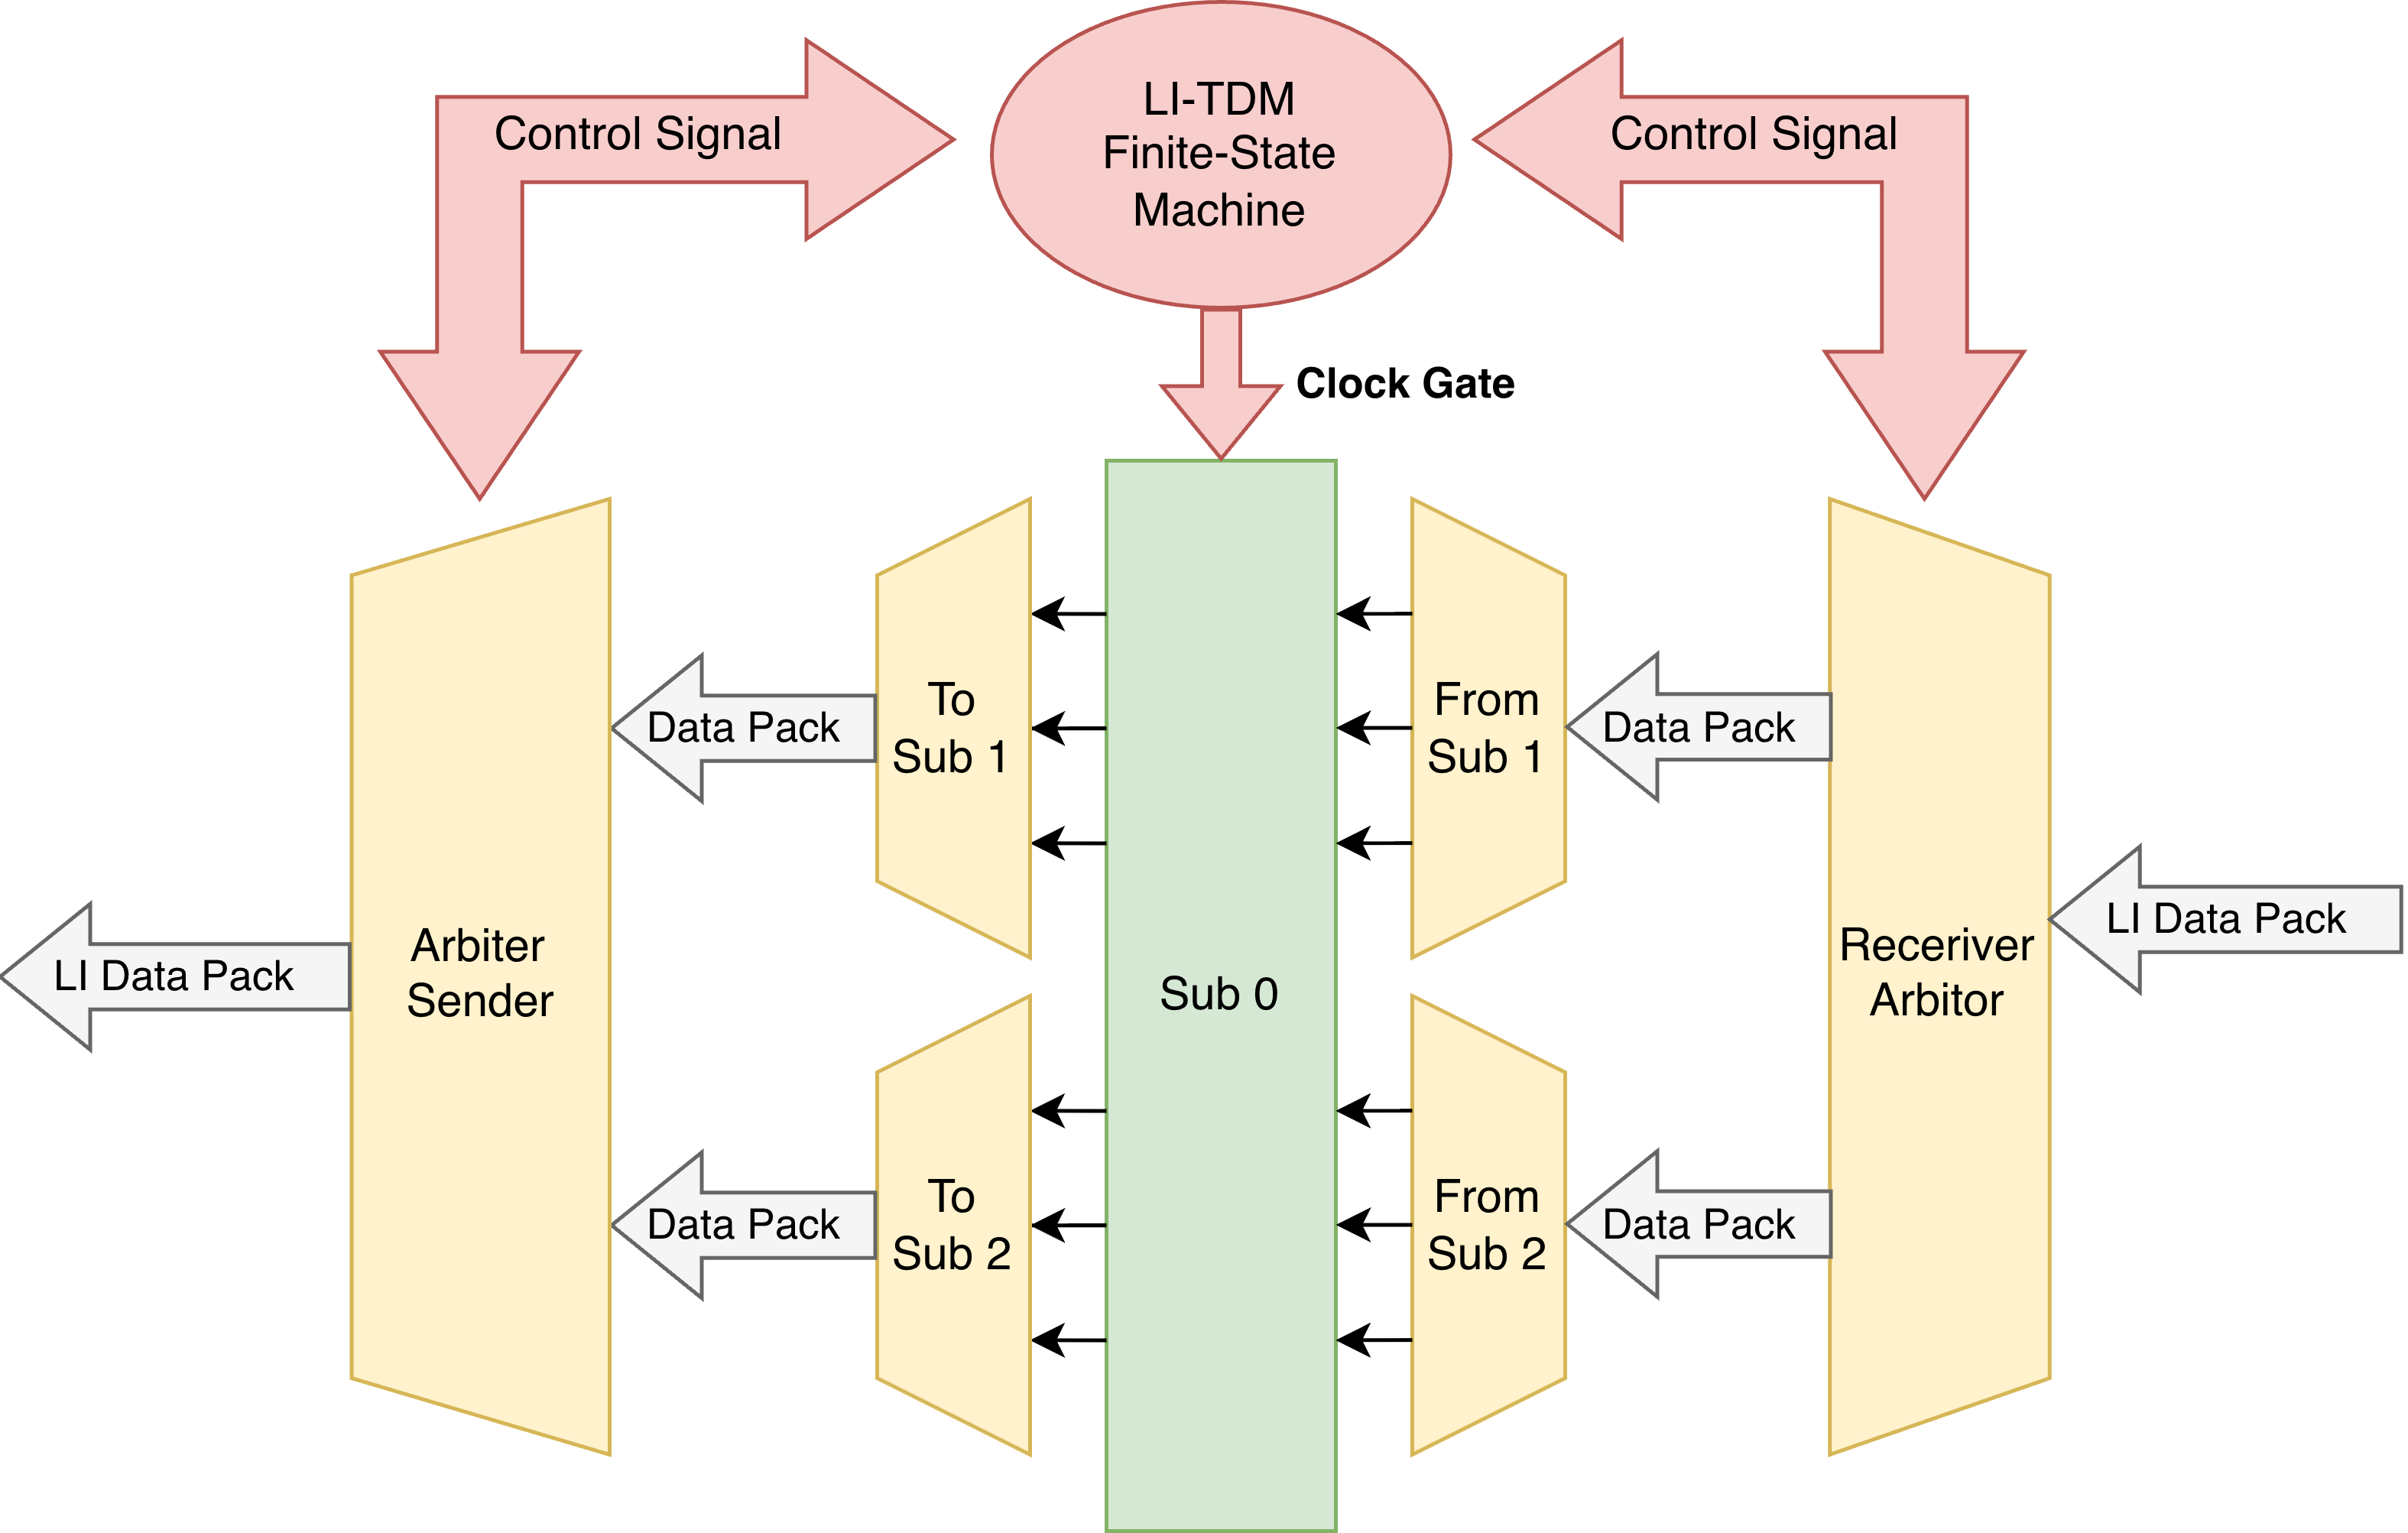
\includegraphics[width=\columnwidth]{figure/LI-TDM.png}
    \bicaption{LI-TDM跨边界接口结构}{LI-TDM cross-boundary interface structure}
    \label{fig::LI-TDM}
\end{figure}

\subsection{物理信道无关的数据平台通信与可扩展的控制平面通信}

划分和后集成，最终部署到多FPGA的计算节点上。计算节点之间互联通信，使各子模块协同工作。前文提到，我们采用AXI Stream协议来实现一种信道无关的流式互联通信。这可以帮助我们在多样化的计算节点与物理互联信道中实现统一互联，增强我们的多FPGA系统的通用性和可扩展性。

在计算节点的组织方式上，REMUS框架将计算节点视作分层架构，存在片内、跨片、和跨服务器三种层级，如图6.1所示。在片内层级，计算节点以运行时层常见的Shell-Role结构组织：每个FPGA加速卡上包含一个Shell，提供配置控制、外设接口等运行时环境，以及多个承载用户逻辑的多个Role。片间层级由多块FPGA加速卡搭配一台主机服务器组成，FPGA可能会由PCIe Switch或者QSFP光纤的方式互联。而在在片间层级，FPGA加速卡通过PCIe接口与主机相连。服务器和加速卡的组合进一步作为基本单元，形成跨服务器层级。在跨服务器层级中，FPGA加速卡和服务器主机都接入数据中心交换机。这一种往往是FPGA云服务的常见部署方式。在上述计算节点的组织架构下，两个计算节点之间存在三种基本的物理互联信道。尽管这些物理信道具有不同的传输协议和物理特性，但大都满足多FPGA系统的通信要求：以数据包形式传输，支持动态路由，具备可靠性。基于这些要求，我们可以将这些物理信道抽象为统一的AXI Stream接口，从而实现跨层级、跨信道的统一互联通信。

AXI Stream的流式互联通信，让物理信道的细节对集成控制器的通信接口透明化，从而简化了计算节点运行时环境的设计。下文介绍运行时环境为用户逻辑提供的丰富控制和通信接口，简化用户逻辑在计算节点上的部署和适配。图6.2展示了硬件逻辑部署到计算节点后的结构，该部署结构同时适用于多种互联信道。整个系统结构包括若干组件，可以分为控制平面和数据平面。数据平面用于传输FPGA跨片数据，该部分前文已经有详细的描述，在此不赘述。控制平面包括三部分：主机上运行的驱动程序、FPGA上的集成控制器、IO通信桥以及连接的相关外设。如表3.1.1所示，三个组件分工协作，在用户逻辑运行的整个周期中都发挥着重要作用。

\begin{table}[htb]
    \centering
    \caption{控制平面功能说明}
    \label{tab::control_plane}
    \begin{tabular}{*{2}{c}}
        \toprule
        运行周期 & 功能说明                        \\
        \midrule
        启动前  & 将软件负载加载到FPGA侧的内存中           \\
        启动时  & 通过扫描链将时序器件的检查点数据导出/导入       \\
        启动后  & 控制设计的启动和暂停                  \\
        启动后  & 改变DUT的输入端口的数据，观察输出端口的数据     \\
        启动后  & 通过串口控制器等外设监控计算节点的运行状态，并与之交互 \\
        \bottomrule
    \end{tabular}
\end{table}

对于发送启停信号，在单片的REMU系统中，主机程序通过PCIe向FPGA上的集成控制器发送写请求，修改内部控制状态寄存器，从而实现控制设计模式切换。在多片的REMUS中，主机驱动程序需要对所有的PCIe设备同时发送写请求，同时修改所有集成控制器的状态。虽然无法保证主机控制程序发送的写请求同时到达每一个集成控制器，但LI-TDM的的设计策略可以保证，他们一定是在完成当前周期的计算之后，才更改内部控制状态寄存器。最终实现所有的子设计全部停止在相同的周期。而对于外设相关的功能，本质上是要求主机驱动程序能够和FPGA上的外设进行交互，这往往也可以通过基于PCIe的DMA或者GPIO来实现。为了简化了外设相关的软件设计，REMUS将I/O通信接口限制在了一个计算节点，其他计算节点只需进行同步的启停操作。除了外设和主机驱动程序的交互，还需要保证外设能和划分逻辑正确的通信，REMUS的运行时环境为划分模块提供了基于AXI的外设接口。需要注意的是外设并不是直接连接到用户逻辑上，而是通过Shell中的I/O通信桥和划分逻辑通信。因为外设运行在计算节点的系统时钟下，而划分逻辑运行在由状态机控制的时钟门控下。I/O通信桥负责在两种时钟域下进行数据传输，并通过FIFO缓冲区实现跨时钟域的数据可靠传输。使得跨时钟域通信对用户逻辑透明化，简化用户逻辑的设计。

\subsection{实验方案及可行性分析}

基于前面章节所提出的研究方法和技术路线，为REMUS设计了相应的实验用于评测REMUS的功能完整性和性能。本节首先介绍多FPGA硬件仿真框架REMUS的具体部署和测试环境，然后介绍各组件的性能测试的实验设计，最后介绍一些端到端的系统试验设计。

对于划分组件的测试，运行的硬件平台是使用Xeon Gold 6338N(128)@3.50GHz处理器核的EDA服务器。划分软件是是基于开源综合工具Yosys 0.52开发的。使用标准的Titian32标准划分数据集以及三个RISC-V开源处理器进行划分实验。评价指标包括切割的组合逻辑数、跳数，以及程序的运行时间。Baseline采用使用相同的超图划分算法KaHyPar、DUOHUAFEN的划分组件，并对比了不同的划分粒度下的划分结果。为了确保划分结果的功能正确性，还会使用形式化验证和逻辑仿真两种方法，测试划分结果没有改变设计的逻辑功能。这种动静结合的测试方法，不光能够有效地发现划分过程中可能引入的错误，还能够快速精确的定位出错现场。加快调试速度，从而确保划分算法正确无误地实现。

集成组件的实验在同样的EDA服务器上进行，使用的FPGA工具链为Xilinx/Vivado2020.2。实验会在相同的划分结果下，对比LI-BDN、LI- TDM跨边界接口电路、REMU扫描链控制单元、REMUS集成控制器的接口电路资源占用和关键路径时序。而在正确性方面，逻辑仿真软件同样是一个重要的保证。首先，需要搭建一个专门多FPGA系统的仿真环境。该仿真环境使用进程间通信来模拟的FPGA之间的数据交换通路，实现跨片数据的传输。使用内存文件映射来模拟PCIe设备在主机通讯节点，实现主机驱动程序和FPGA之间的控制通路。完备的逻辑仿真可以尽可能减少上板时出现的异常情况，提高项目的可行性。

对于通信实验，计划部署了如下的异构FPGA系统：使用多张课题组内自建的FPAG板卡——NewMemory，基于VU37P FPGA芯片。测试和评估在一台主机服务器内，通过PCIe物理信道使两个FPGA芯片上的计算节点协同工作。在具体的组织形式上，两张加速卡搭配一台主机服务器，通过PCIex16接口将加速卡与服务器连接。跨片数据通过主机进行转发。我们还实现了基于QSFP或高速以太网物理信道的跨节点通信。

最后，本项目计划搭建一个多FPGA和x86主机的松耦合异构计算平台，预计最终实现4个FPGA和一台主机的互联。该平台上会部署了多个RISC-V处理器核，运行相同benchmark，对比了不同物理信道和时钟频率下的逻辑时钟频率和运行裸机程序的性能。